\chapter{Marco teórico}
\label{ch:marco}

\begin{comment}
\section{Descripción}

Para comprender el tema ADAS es necesario manejar una serie de definiciones y conocer contextualmente la Visión por Computadora, el Control Automático así como la gran variedad de aplicaciones ADAS que se están incluyendo en los vehículos que existen en el mercado actualmente. 

\vspace{-0.5cm}

\section{Antecedentes}

La automatización de la conducción no solo viene inspirada en crear vehículos inteligentes, si no que con esa autonomía se puedan eliminar los números rojos que existen debido a muertes y accidentes automovilísticos en las carreteras y caminos de todo el mundo. En Costa Rica los números son alarmantes.

Los accidentes automovilísticos fueron, en Costa Rica, la tercera causa en el 2015 de muertes\cite{Rodriguez2016}. Según datos de la Policía de Tránsito, el año anterior (2016) se contabilizaron 448 muertes por accidentes de tránsito; es decir, 60 más que en el 2015, 93 más que en el 2014. Y más preocupante aún es saber que el recuento que hace la Policía de Tránsito solamente incluye las muertes en el sitio. No toma en cuenta a quienes tuvieron un accidente, pero fallecieron en los centros médicos. Las colisiones entre vehículos son el tipo de accidentes que cobran más vidas, con 213 muertes, lo cual representa un 47\%.Otras causas como atropellos dejaron 70 fallecimientos; autos que se salieron de la vía, 70; vuelcos, 32; choques contra objetos fijos, 31; derrapes, 14; atropellos en los que el responsable se dio a la fuga, 14, y 4 conductores que se quedaron dormidos \cite{Bosque2017}.





\subsection{Automóviles}

one in five of the nearly three million newly registered passenger cars in Germany last year were equipped with ADAS. Bosch, december 22, 2015 Stuttgart

%Read more at http://telematicswire.net/half-of-the-drivers-prefer parking-assist-adas-feature-in-new-connected-vehicles-bosch/#gIKq 3RmquPTWLM0.99
\end{comment}





%----OReilly Learning OpenCV.pdf paginas 2-3-----

%\subsection{Visión en Industria automotriz}

%Describirlo muy general




\section{Generalidades}
\subsection{Niveles de Autonomía en Vehículos}

La Sociedad de Ingenieros de Automoción (\textit{Society of Automotive Engineers}, SAE) en la norma J3016 establece una serie de definiciones y clasificaciones con el fin de que se tenga una terminología en común entre industria, academia y todos los involucrados en lo relacionado a conducción autónoma. Se expone, en dicha norma, una clasificación por niveles para el nivel de autonomía al conducir, partiendo de nivel cero el cual afirma que el vehículo posee autonomía de conducción nula hasta llegar a un nivel cinco que asegura que el vehículo puede ser conducido por si mismo sin necesidad de un conductor.
Esta clasificación mencionada es importante para mantener a todos los sectores, que tienen las ADAS en discusión, alineados y erradicar confusiones sobre en que nivel de conducción autónoma se encuentra cierto objeto de estudio\cite{SAE2016}. 

%--------------------Agregar la imagen de la pagina 1 del pdf de la SAE-------------

\subsubsection{Nivel 0. Automatización Inexistente}
\begin{myindentpar}{5cm}
El nivel 0 viene dado por cero asistencia y cero autonomía de manejo. Toda la dinámica de conducción es ejecutada por un conductor humano. En este nivel no existen los modos de manejo ni el control de aumento o descenso de velocidad.
\end{myindentpar}

\subsubsection{Nivel 1. Asistencia al Conductor}
\begin{myindentpar}{5cm}
 {El nivel 1 es apoyado por modos de conducción, asistencia de aceleración y desaceleración. Se le da al conductor libertar de pies por lo que en ingles se le conoce a este nivel como ``Feet-off".}
\end{myindentpar}

\subsubsection{Nivel 2. Automatización Parcial}
\begin{myindentpar}{5cm}
{El vehículo posee varios sensores para obtener datos del entorno y el control de velocidad, por su parte, ya es parte del control del sistema y posee variedad modos de conducción. Por lo anterior, en este nivel se le da libertad al conductor de manos y debido a ello se le conoce en ingles como ``Hands-off".}
\end{myindentpar}

\subsubsection{Nivel 3. Automatización Condicional}
\begin{myindentpar}{5cm}
{El sistema se encarga de lo que concierne la conducción pero solicita intervención del chofer en ocasiones. Se le conoce como ``Eyes-off" o Ojos libres pues le da la libertad al conductor de realizar tareas en las cuales necesite su visión sin afectar la conducción del vehículo. }
\end{myindentpar}

\subsubsection{Nivel 4. Automatización Elevada}
\begin{myindentpar}{5cm}
{No es necesaria la intervención del usuario ya que el vehículo cuenta con las herramientas de hardware y software necesarias para ser conducido por sí solo y el conductor este únicamente para casos excepcionales. A este nivel debido a lo mencionado se le conoce como ``Brain-off" o Mente libre.}
\end{myindentpar}

\subsubsection{Nivel 5. Automatización Total}
\begin{myindentpar}{5cm}
{Para esta instancia el vehículo toma en cuenta entorno y todos los aspectos de la dinámica de manejo. Por ello no es necesario el conductor humano.}
\end{myindentpar}

La Sociedad Internacional de Ingenieros Automotrices en \cite{SAE2016} plantea que existen, más allá de los distintos niveles, una división general que comprende 2 grupos que abarcan 3 niveles de autonomía cada uno. 

\begin{itemize}
    \item {El conductor humano controla el ambiente de conducción}
    
    En el cual los niveles 0, 1 y 2 se ven representados.
\end{itemize}
\begin{itemize}
    \item {Sistema de conducción automatizado controla el ambiente de conducción}
    
    Los niveles 3, 4 y 5 forman parte de esta división.
\end{itemize}
\begin{figure}[H]
  \centering
  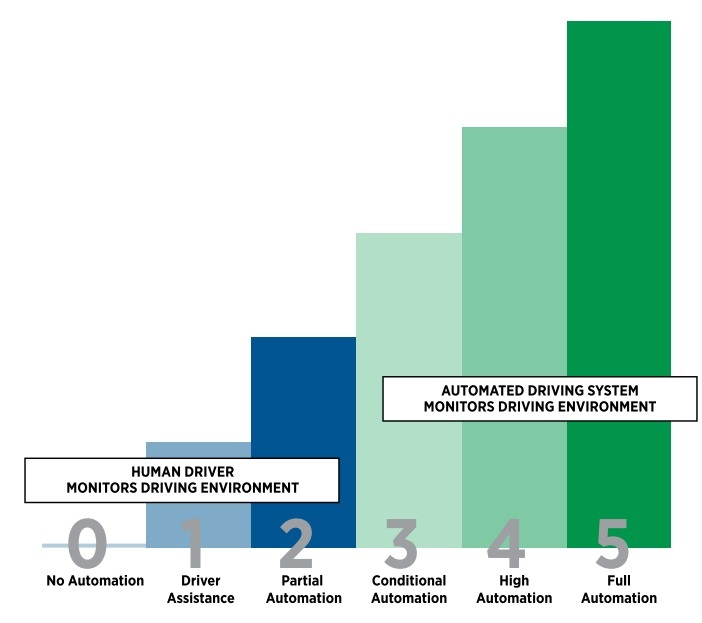
\includegraphics[width=0.65\textwidth]{bardiagram}
  \caption{Representación gráfica de niveles.}
  \label{fig:boat1}
\end{figure}

Lo que se busca con estas aplicaciones ADASs es proveer de herramientas a la industria automotriz para lograr ese ansiado Nivel 5 de autonomía y conseguir que el AD sea toda una realidad.



\subsection{Sensores en ADAS}

Las aplicaciones ADAS requieren mediciones variadas de variables físicas del entorno que rodea los vehículos. Esta información viene dada por distintos sensores que se describen a continuación.

\subsubsection{Cámaras Monoculares}

Si se tiene un solo sensor de cámara para captura de video que necesita ser procesado y analizado, en este caso se habla de un Sistema Monocular también llamado ``Single-Eyed System" y permite obtención de imágenes en 2 dimensiones\cite{Dubey2016}.

Estas sensores son recomendados en \cite{Dubey2016} para: 
\begin{multicols}{3}
\begin{itemize}
    \item {Líneas}
\end{itemize}
\begin{itemize}
    \item {Peatones}
\end{itemize}
\begin{itemize}
    \item {Señales de transito}
\end{itemize}
\end{multicols}

\vspace{-0.50cm}
\subsubsection{Cámaras Stereo}

Un sistema con dos cámaras, separadas una de otra se llama Sistema de Stereo Visión. El costo de este tipo de sensor es 1.5 veces el de un sensor monocular. Los sensores deben estar un mínimo 25-30cm separados entre sí para obtener imágenes en 3 dimensiones\cite{Dubey2016}.

Estas sensores son recomendados en \cite{Dubey2016} para: 
\begin{multicols}{2}
\begin{itemize}
    \item {Detección de objetos}
\end{itemize}
\begin{itemize}
    \item {Cálculo de distancia}
\end{itemize}
\end{multicols}

\vspace{-0.50cm}
\subsubsection{Cámaras Infrarrojas}

Existen aplicaciones de visión artificial que requieren soluciones más allá del espectro visible, debido a las características de emisión de los objetos o de la aplicación a evaluar. Para ello existen las cámara infrarrojas y como se explica en \cite{Alava2010} la radiación
infrarroja está comprendida entre las fracciones visible y de microondas del espectro electromagnético. 
Existen 2 clasificaciones principales para estos sensores brindada por \cite{Kallhammer2006}, NIR y FIR. Los sistemas NIR poseen alta resolución y menor rango de alcance que los FIR además de que perciben radiación en el limite del rango visible. Estos segundos tienen, por su parte poseen mejor desempeño en la detección un ejemplo de ellos es la detección de transeúntes y objetos y es utilizado por marcas como la BMW, Mercedes-Benz y Honda para su sistema de Visión Nocturna ya que detectan la radiación que los peatones emiten.  


\subsubsection{Ultrasonido}

Un sensor ultrasónico transmite ondas ultrasónicas en el aire y detecta ondas reflejadas de un objeto. Hay muchos usos para los sensores ultrasónicos, por ejemplo en sistemas de alarma de la intrusión, los accesos automáticos y los sensores de la retroceso para los automóviles. Acompañado por el rápido desarrollo de la tecnología de procesamiento de información, nuevos campos de aplicación, tales como equipos de automatización de fábrica y electrónica de automóviles, están aumentando y deben seguir haciéndolo\cite{Manual2008}.


\subsubsection{LIDAR}

Los sistemas de Detección y Alcance de Luz (\textit{Light Detection And Ranging},LIDAR) utilizan el mismo principio que el radar se desarrollan para una amplia gama de aplicaciones de localización, de rango y de generación de perfiles. Tal sistema consiste en un láser capaz de transmitir la luz (pulsada o continua) sobre la gama de interés requerida, y un receptor de alta velocidad, de poco ruido para el análisis reflejado de la señal. La luz transmitida interactúa y es cambiada por el objetivo. 
un porcentaje de esta luz se refleja/se dispersa de nuevo al receptor según la reflectividad del blanco. Los cambios en las propiedades de la señal transmitida permiten determinar algunas propiedades del destino. En la aplicación más común, el Tiempo de Vuelo (\textit{Time of Flight}, TOF) se utiliza para determinar el rango. A medida que la tecnología analógica mejora el rendimiento y la disponibilidad, la tecnología LiDAR sigue encontrando su camino en aplicaciones más y más emocionantes.\cite{Ha2015}


\begin{comment}

\subsubsection{Varios}

----Figura 1. pagina 50 Scanning LIDAR 0753.......------


---Table 1.A  A comparison........   page 51 Scanning LIDAR 0753.......------

-----Ver tabla 8 pagido 110 Embeddubg vision-based07921..pdf-----

\end{comment}

En la Figura 2.2 se muestra de manera gráfica y descriptiva el alcance de los distintos tipos de sensores que se utilizan para las distintas aplicaciones ADAS.

\begin{figure}[H]
  \centering
  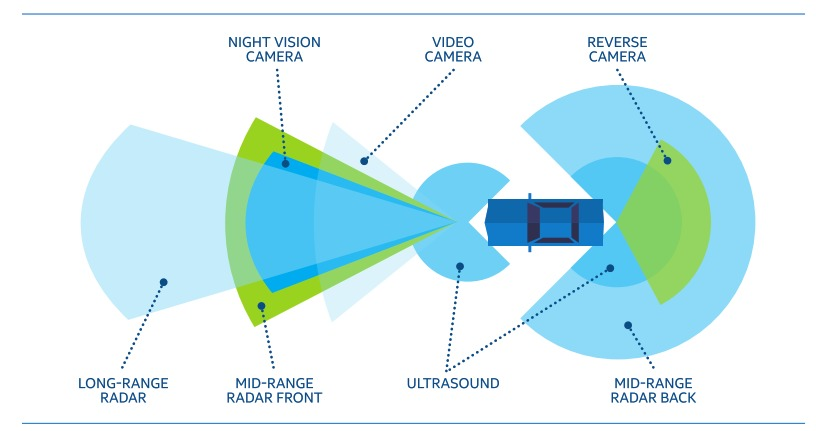
\includegraphics[width=0.85\textwidth]{carsensors.jpeg}
  \caption{Alcance de sensores.}
  \label{fig:boat2}
\end{figure}

\section{Taxonomía}
\index{Tax}

Intel propone en \cite{Intel2016} una clasificación para las aplicaciones ADAS que se pueden encontrar en los distintos modelos de vehículos que hay en el mercado. Esto para facilitar su comprensión y estudio. 

Inicialmente propone dividirlo en 6 grandes ramas las cuales son:
\begin{multicols}{3}

\begin{itemize}
    \item {Estabilidad de
    
    Conducción}
\end{itemize}
\begin{itemize}
    \item {Control Longitudinal}
\end{itemize}
\begin{itemize}
    \item {Apoyo en Cabina}
\end{itemize}
\begin{itemize}
    \item {Control Lateral}
\end{itemize}
\begin{itemize}
    \item {Apoyo al Estacionar}
\end{itemize}
\begin{itemize}
    \item { Luz y Vista}
\end{itemize}

\end{multicols}

Con la finalidad de profundizar el tema y conocer las principales aplicaciones ADAS dentro de las familias mencionadas anteriormente. Para cada ADAS se presenta su nombre, su acrónimo, una breve descripción y finalmente los sensores que se utilizan para cumplir con su función.  

\newpage

\subsection{Estabilidad de Conducción}

En esta primera división se presentan las ADAS que le permiten al conductor conducir sin preocuparse de que el vehículo vaya a tener inconvenientes movilizandose sobre distintos tipos de terrero o que se pierda el control al momento de frenado.

\subsubsection{Control de Tracción {\footnotesize(\textit{Traction Control System}, TCS)}}

Prevenir la pérdida de adherencia de las ruedas no patinen cuando el conductor se excede en la aceleración del vehículo o el suelo está muy deslizante el sistema actúa con el fin de reducir el par de giro y así recuperar la adherencia entre neumático y firme, realizando una (o más de una a la vez) de las siguientes acciones, en primer lugar retarda o suprime la chispa a uno o más cilindros. Seguidamente, reduce la inyección de combustible a uno o más cilindros. Para finalmente frenar la rueda que ha perdido adherencia. Los sensores utilizados son generadores de pulsos ubicados en las ruedas del vehículo.

\subsubsection{Control Electrónico de Estabilidad {\footnotesize(\textit{Electronic Stability Control }, ESC)}}

Este sistema utiliza el frenado automático de las ruedas individuales para evitar que el título cambie demasiado rápido (derrapando) o no lo suficientemente rápido (trabandose). ESC no puede aumentar la tracción disponible, pero maximiza la posibilidad de mantener el vehículo bajo control y en la carretera durante maniobras extremas utilizando la reacción natural del conductor de dirección en la dirección prevista\cite{Hospach2014}.ESC pasa tan rápido que los conductores no perciben la necesidad de correcciones de dirección. Si los conductores se frenan porque la curva es más o menos aguda de lo previsto, el sistema sigue siendo capaz de generar frenado desigual si es necesario para corregir el rumbo. Utiliza sensores de velocidad y ángulo y acelerómetros.

\subsection{Control Longitudinal}

El Control Longitudinal le brinda al conductor herramientas para que la conducción en carreteras sea más sencilla y segura.

\subsubsection{Control Automático de Crucero {\footnotesize(\textit{Automatic Cruise Control}, ACC)}}

Esta es la versión avanzada de la función actual de control velocidad crucero. Actualmente, el control de velocidad crucero acepta un valor ajustado de velocidad desde el controlador y gestiona el sistema de control del vehículo para mantener la velocidad de destino. Puede tomar la información adicional de la detección para la gerencia de la velocidad del camino, arriba/abajo de la colina y las curvas del camino. Sin embargo, el control tradicional de cruceros no permite que el vehículo ajuste la velocidad del vehículo de forma dinámica según la distancia relativa. El ACC permite un ahorro de combustible al mantener un manejo a velocidad constante y le permite adicionalmente al conductor descansar sus pies \cite{Thakur2016}. Esta aplicación requiere de cámaras monoscópicas, sensores de velocidad y sistemas LiDAR.


\subsubsection{Asistente Inteligente de Velocidad {\footnotesize(\textit{Intelligent Speed Assistance}, ISA)}}

Los sistemas de ISA establecen la posición de un vehículo y comparan la velocidad del vehículo con el límite de velocidad fijado en una ubicación dada usando mapas digitales o signos de límite de la velocidad de lectura como una base. Los sistemas entonces dan la reacción en el vehículo sobre ese límite de velocidad al conductor o hasta restringen la velocidad del vehículo según el límite de velocidad vigente \cite{Swov2008}. Precisan de entradas de video, radar y sistemas LiDAR.

\subsubsection{Reconocimiento de Señales de Transito {\footnotesize(\textit{Traffic Sign Recognition}, TSR)}}

Consiste principalmente en la detección de señales de tráfico de tecnología básica y la identificación de localización. Los métodos de detección de señales de tráfico son principalmente basados en color o en forma o el método de combinar esos dos. Hay muchas investigaciones sobre la detección e identificación basada en el color, como la detección de bordes de color para cada canal de espacio de color, el separatismo regional, la segmentación de umbrales y la agrupación. A los métodos basados en la forma de la detección y de la identificación, hay método de la codificación gráfica, el método de la transformación de Hough, el método que empareja de la plantilla etc \cite{Wang2010}. Con el uso de cámaras monoscópicas se obtiene la data de entrada al sistema.

\subsubsection{Reconocimiento de Luces de Transito {\footnotesize(\textit{Traffic Signal Lamp Recognition}, SLR)}}

Es crítico para detectar rápidamente y con precisión los semáforos y eliminar el ruido de la escena para detectar y reconocer los semáforos. En esta interviene la luz del sol que al no ser constante en el tiempo entorpece la toma de datos, siendo este uno de los mayores problemas.\cite{Wang2017}. Las cámaras monoscópicas son las utilizadas para esta aplicación. 

\subsubsection{Freno Automático de Emergencia {\footnotesize(\textit{Automatic Emergency Brake}, AEB)}}

Este sistema es de los uno de los más importantes de los ADAS y de este dependen muchos otros como, CAS, PPS, ACC, DDS, etc. Lo que realiza es enviar la señal a los frenos para que se accionen automaticamente según las circunstancias para evitar colisiones\cite{Hosseini2016}. Los sensores utilizados son cámaras, sensores de velocidad y sistemas LiDAR. 

\newpage

\subsubsection{Control de Alerta de Peatones {\footnotesize(\textit{Pedestrian Protection System}, PPS)}}

Lo que se plantea con esta aplicación es detectar transeúntes sobre la ruta del vehículo mediante CV. Esto para evitar accidentes de transito en los que se atente directamente la integridad de un eventual peatón. Una vez detectado se trabaja en conjunto con otras ADAS como CAS o AEB para poder cumplir su objetivo \cite{Kuo2016}. Para la detección de peatones las cámaras y los sistemas ultrasonido así como sistemas LiDAR y sistemas infrarojos.


\subsubsection{Alerta Pre-Colisión {\footnotesize(\textit{Pre-Collision Warning}, PCW)}}

Los sistemas que pueden detectar y alertar al conductor para que accidentes inminentes se conocen como sistemas pre-colisión. El sistema tensa los cinturones de seguridad y realiza un frenado de la paulatino. En primer lugar activa una alerta visual o sonora y cierra las ventanas, luego activa un frenado suave para captar la atención de conductor, seguidamente aplica un freno que provoque mayor reducción de velocidad, para finalmente frenar con todo poder\cite{Thakur2016}. Los sistemas aparecieron por primera vez a mediados de los 2000 por Toyota y Honda. Los sistemas LiDAR y las cámaras son de donde la PCW obtiene la información necesaria para realizar su función. 

\subsubsection{Sistema de Evasión de Colisiones {\footnotesize(\textit{Collision Avoidance System}, CAS)} }

El sistemas anti-colisión por frenado (PCW) es apropiado a velocidades bajas del vehículo y de evasión de colisión por la dirección es más apropiado a velocidades más altas. La mayoría de los sistemas de evitación de colisiones de automóviles atraen tecnologías existentes. Dado que estos sistemas requieren sensores frontales, a menudo sacan datos de los mismos sensores que utilizan un sistema de control de cruceros adaptativo. Si el diferencial de velocidad entre el vehículo y cualquier objeto frente a él es demasiado grande, entonces el sistema puede ser capaz de realizar un puñado de tareas diferentes. Los sistemas más simples de la evitación de la colisión emitirán una advertencia en este punto, que con suerte proporcionará el conductor con suficiente ADVERTENCIA avanzada para golpear los frenos o alejarse de la obstrucción o bien algunos sistemas de evitación de colisiones de automóviles también son capaces de tomar medidas directas y correctivas \cite{PintoNeto2016}. Los sensores que se utilizan son radar, LiDAR y una cámara frontal. 

\newpage

\subsection{Control Lateral}

El Control Lateral le provee al conductor las herramientas necesarias para realizar cambios de carril de manera segura. 

\subsubsection{Detección de Punto Ciego {\footnotesize(\textit{Blind Spot Detection}, BSD)}}

Los puntos ciegos son áreas fuera de un vehículo que el conductor es incapaz de ver. Los puntos ciegos pueden ser causados por los pilares de la ventana, reposacabezas, pasajeros y otros objetos. A distancias incluso moderadas, un punto ciego causado por un pilar a puede oscurecer objetos grandes como los coches y las personas. Otro tipo de punto ciego vehicular existe en el espacio entre la visión periférica del conductor y el área reflejada por los espejos retrovisor. Este tipo de punto ciego puede tragar vehículos enteros, por lo que es tan peligroso cambiar de carril sin mirar a la izquierda o a la derecha. Este sistema genera una alerta según sea la proximidad del objeto al punto siego sensado \cite{Thakur2016}.Los sensores que generalmente se utilizan son cámaras para obtener una vision 360 grados del carro y radares. 

\subsubsection{Alerta de Salida del Carril  {\footnotesize(\textit{Lane Departure Warning}, LDW)}}

Los sistemas de alerta de salida de carril son un grupo de tecnologías de seguridad que están diseñados principalmente para evitar la alta velocidad de los accidentes en carreteras y autopistas.Al advertir al conductor, o incluso tomar acciones correctivas automáticas, estos sistemas son capaces de prevenir muchas colisiones y accidentes de carretera. Según \cite{Otaegui2016} los algoritmos LDW son junto con TSR los más estudiados y de baja complejidad computacional. Las cámaras son los sensores utilizados para este fin. 

\subsubsection{Asistente de Cambio de Carril {\footnotesize(\textit{Lane Change Assistance}, LCA)}}

Los cambios del carril son maniobras estresantes para los conductores, particularmente durante flujos de alta velocidad del tráfico. Los sistemas avanzados de asistencia al conductor tienen como objetivo ayudar a los conductores durante las maniobras de cambio de carriles. Un sistema que se desarrolla para un conductor medio o todos los conductores tendrá que ser conservador por razones de seguridad para cubrir todos los tipos de conductor/vehículo. Tal sistema conservador puede no ser aceptable a los conductores agresivos y se podría percibir como demasiado agresivo por los conductores más pasivos. Un ADAS que tenga en cuenta las dinámicas y características de cada sistema individual de vehículo/conductor durante las maniobras de cambio de carriles será más eficaz y más aceptable para los conductores sin sacrificar la seguridad \cite{Butakov2015}. Las entradas de esta aplicación son los datos obtenidos por BSD y LDW.

\newpage

\subsection{Apoyo en Cabina}

El apoya en cabina le brinda al conductor facilidades tanto de localización de lugares a donde desee ir y posición actual como de alerta ante cansancio del mismo. 

\subsubsection{Sistema de Navegación {\footnotesize(\textit{Navigation System}, NS)}}

Permite conocer la posición del vehículo y el lugar de destino. Con esto generar rutas para que el conductor se movilice de un punto A a un punto B con todas las indicaciones necesarias para realizarlo de manera exitosa. El GPS es la entrada que le permite al sistema conocer la localización del vehículo de manera precisa.

\subsubsection{Monitoreo del Estado del Conductor {\footnotesize(\textit{Driver State Monitoring}, DSM)}}

Los sistemas de alerta de los conductores están estrechamente relacionados con los sistemas de alerta de salida de carril, en que la mayoría de ellos funcionan manteniendo la pista visual de las marcas de carriles para identificar cualquier desviación del carril. Mientras que los sistemas de advertencia de salida de carril están diseñados para prevenir la desviación bajo cualquier circunstancia, los sistemas de alerta de los conductores están específicamente orientados a identificar signos de fatiga del conductor. En \cite{Velez2015} se expone otro sistema que va un paso más allá, monitorizando los ojos y la cara del conductor para ver si hay signos de somnolencia. Si el sistema determina que el conductor tiene problemas para permanecer despierto, puede tomar medidas correctivas. Esto mediante una cámara colocada en el tablero del vehículo.

%-----REVISAR %https://one.nhtsa.gov/people/injury/drowsy_driving1/drowsy.html

\subsection{Apoyo al Estacionar}

La tarea de estacionar en ocasiones no es sencillo pero estas aplicaciones le brindan apoyos al conductor para realizar esta tarea de manera fácil, rápida y precisa.

\subsubsection{Cámara Visión Trasera {\footnotesize(\textit{Rear View Camera}, RVC)}}

Brinda apoyo al conductor al momento de conducir en reversa, principalmente cuando se estaciona en reversa. Este sistema puede ser con cámaras monoculares, stereos o una composición de las anteriores para generar una visión 360 grados del vehículo y poder observar todo alrededor. Este sistema contempla funciones básicas de transmisión en tiempo real de lo que la cámara de retroceso graba pero no interviene ni genera alarmas \cite{Park2017}. 

\newpage

\subsubsection{Asistencia Inteligente de Parqueo  {\footnotesize(\textit{Intelligent Parking Assistance}, IPA)}}

El sistema de asistencia para el estacionamiento ayuda al conductor a dirigir y revisar la parte trasera para asegurarse de que el área esté despejada al hacer retroceder el vehículo. 
Cuando un conductor pone un vehículo en reversa para entrar en un espacio de estacionamiento, el sistema de asistencia de estacionamiento muestra los dos tipos de información. En primer lugar una imagen tomada por un sensor de imagen (colocado en el techo trasero del vehículo), que incluye puntos de vista que no pueden ser vistos por el conductor. En segundo lugar Se le despliega al conductor una imagen superpuesta en la imagen original indicándole una curva con la dirección que debe de tomar \cite{Reyher2010}. El ultrasonido y las cámaras son los que brindan la información necesaria para que esta ADAS funcione.


\subsection{Luz y Vista}

\subsubsection{Visión Nocturna {\footnotesize(\textit{Night Vision}, NV)}}

Como los peatones y los animales tienen el mayor riesgo de aumento en el tráfico nocturno debido a la oscuridad, la capacidad de detectar esos objetos debe ser el principal criterio de rendimiento, y el sistema debe seguir siendo eficaz cuando se enfrenta a los faros de vehículos que se avecinan. El sistema infrarrojo lejano se ha demostrado para ser superior al sistema infrarrojo cercano en términos de distancia peatonal de la detección \cite{Reyher2010}. Los sensores utilizados son FIR.

\subsubsection{Sistema Adaptativo de Luces Frontales  {\footnotesize(\textit{Adaptative Frontlight System}, AFS)} }

El Sistema Adaptativo de Luces Frontales es una parte del sistema de seguridad activo de un vehículo de gama media alta, proporcionando una visión optimizada al conductor durante la noche y otras condiciones de la mala vista de la carretera adaptando el ángulo y la intensidad de la linterna, y juzgando la velocidad del coche, del ángulo del volante, de la condición atmosférica, y de la velocidad del desvío y de la inclinación del coche\cite{INSTRUMENTS2013}. Para este sistema adaptativo de faros se necesita conocer la velocidad del vehículo y los datos brindados por LDW.

\newpage

\subsubsection{Sistema de Sensado de Lluvia {\footnotesize(\textit{Rain Sensor System}, RRS)}}

El sensor de lluvia está instalado en el parabrisas en una sección del mismo con una tasa de transmitancia determinada para permitir el paso de la intensidad especificada de la radiación. La sección de emisión de la unidad del sensor de lluvia emite rayos infrarrojos contra el parabrisas y luego detecta la cantidad de gotas de lluvia al recibir rayos reflejados con fotodiodo. La sección de detección en el parabrisas se encuentra justo por encima del punto central entre el LED y el fotodiodo \cite{Wiper2004}. Los fotodiodos son los que se encargan de detectar si entre el emisor y el receptor hay suficiente paso de luz. Si debido la refracción generada por las gotas el receptor no percibe el haz emitido por el emisor las escobillas realizan su función de manera automática. 

\newpage

\section{Tabla Resumen}

En la sección 2.3 se presentó la recopilación realizada acerca de las ADAS existentes hasta el 2017. Lo que se muestra en la Tabla 2.1 es un resumen de la información expuesta en dicha sección. En esta tabla se muestra la familia a la que pertenece, el nivel de autonomía que aporta así como los sensores que utiliza.  
\begin{table}[H]
\centering
\caption{Tabla Resumen}
\label{my-label}
\begin{tabular}{|l|c|c|c|c|}
\hline
\multicolumn{1}{|c}{Familia} & \multicolumn{1}{|c}{ADAS} & \multicolumn{1}{|c|}{\begin{tabular}[c|]{@{}c@{}}Nivel de \\ Autonomía\end{tabular}} & Sensores \\ \hline

Est Cond                      & TCS                       & 2                                                                                  & Velocidad    \\ 
Est Cond                      & ESC                       & 2                                                                                   & Acelerómetro-Ángulo-Velocidad           \\ 
Ctr Long                      & ACC                       & 3                                                                                   & Cámara-Velocidad-LiDAR          \\ 
Ctr Long                      & ISA                       & 3                                                                                   & Cámara-Radar-LiDAR          \\ 
Ctr Long                      & TSR                       & 1                                                                                  &   Cámara          \\
Ctr Long                      & SLR                       & 1                                                                                   &  Cámara         \\ 
Ctr Long                      & AEB                       & 3                                                                                   &     Velocidad-Cámara        \\ 
Ctr Long                      & PPS                       & 3                                                                                   &   Cámara        \\ 
Ctr Long                      & PCW                       &  3                                                                                  &     LiDAR-Cámara        \\ 
Ctr Long                      & CAS                       &  3                                                                                  &     Cámara-Radar-LiDAR        \\ 
Ctr Lat                       & BSD                       & 1                                                                                   &     Cámara-Radar     \\ 
Ctr Lat                       & LDW                       & 2                                                                                    &     Cámara     \\ 
Ctr Lat                       & LCA                       & 2                                                                                   &     Cámara-Radar-LiDAR     \\ 
Apy Cab                       & NS                        & 1                                                                                   &     GPS     \\ 
Apy Cab                       & DSM                       & 2                                                                                   &      Cámara    \\ 
Apy Est                       & RVC                       & 1                                                                                  &      Cámara    \\ 
Apy Est                       & IPA                       & 1                                                                                   &      Cámara-Ultrasonido    \\ 
Luz Vis                       & NV                        & 1                                                                                   &     FIR     \\ 
Luz Vis                       & AFS                       & 3                                                                                  &       Cámara-Velocidad   \\
Luz Vis                       & RSS                       & 3                                                                                   &      Fotodiodo    \\  \hline
\end{tabular}
\end{table}
